\documentclass[1p]{elsarticle_modified}
%\bibliographystyle{elsarticle-num}

%\usepackage[colorlinks]{hyperref}
%\usepackage{abbrmath_seonhwa} %\Abb, \Ascr, \Acal ,\Abf, \Afrak
\usepackage{amsfonts}
\usepackage{amssymb}
\usepackage{amsmath}
\usepackage{amsthm}
\usepackage{scalefnt}
\usepackage{amsbsy}
\usepackage{kotex}
\usepackage{caption}
\usepackage{subfig}
\usepackage{color}
\usepackage{graphicx}
\usepackage{xcolor} %% white, black, red, green, blue, cyan, magenta, yellow
\usepackage{float}
\usepackage{setspace}
\usepackage{hyperref}

\usepackage{tikz}
\usetikzlibrary{arrows}

\usepackage{multirow}
\usepackage{array} % fixed length table
\usepackage{hhline}

%%%%%%%%%%%%%%%%%%%%%
\makeatletter
\renewcommand*\env@matrix[1][\arraystretch]{%
	\edef\arraystretch{#1}%
	\hskip -\arraycolsep
	\let\@ifnextchar\new@ifnextchar
	\array{*\c@MaxMatrixCols c}}
\makeatother %https://tex.stackexchange.com/questions/14071/how-can-i-increase-the-line-spacing-in-a-matrix
%%%%%%%%%%%%%%%

\usepackage[normalem]{ulem}

\newcommand{\msout}[1]{\ifmmode\text{\sout{\ensuremath{#1}}}\else\sout{#1}\fi}
%SOURCE: \msout is \stkout macro in https://tex.stackexchange.com/questions/20609/strikeout-in-math-mode

\newcommand{\cancel}[1]{
	\ifmmode
	{\color{red}\msout{#1}}
	\else
	{\color{red}\sout{#1}}
	\fi
}

\newcommand{\add}[1]{
	{\color{blue}\uwave{#1}}
}

\newcommand{\replace}[2]{
	\ifmmode
	{\color{red}\msout{#1}}{\color{blue}\uwave{#2}}
	\else
	{\color{red}\sout{#1}}{\color{blue}\uwave{#2}}
	\fi
}

\newcommand{\Sol}{\mathcal{S}} %segment
\newcommand{\D}{D} %diagram
\newcommand{\A}{\mathcal{A}} %arc


%%%%%%%%%%%%%%%%%%%%%%%%%%%%%5 test

\def\sl{\operatorname{\textup{SL}}(2,\Cbb)}
\def\psl{\operatorname{\textup{PSL}}(2,\Cbb)}
\def\quan{\mkern 1mu \triangleright \mkern 1mu}

\theoremstyle{definition}
\newtheorem{thm}{Theorem}[section]
\newtheorem{prop}[thm]{Proposition}
\newtheorem{lem}[thm]{Lemma}
\newtheorem{ques}[thm]{Question}
\newtheorem{cor}[thm]{Corollary}
\newtheorem{defn}[thm]{Definition}
\newtheorem{exam}[thm]{Example}
\newtheorem{rmk}[thm]{Remark}
\newtheorem{alg}[thm]{Algorithm}

\newcommand{\I}{\sqrt{-1}}
\begin{document}

%\begin{frontmatter}
%
%\title{Boundary parabolic representations of knots up to 8 crossings}
%
%%% Group authors per affiliation:
%\author{Yunhi Cho} 
%\address{Department of Mathematics, University of Seoul, Seoul, Korea}
%\ead{yhcho@uos.ac.kr}
%
%
%\author{Seonhwa Kim} %\fnref{s_kim}}
%\address{Center for Geometry and Physics, Institute for Basic Science, Pohang, 37673, Korea}
%\ead{ryeona17@ibs.re.kr}
%
%\author{Hyuk Kim}
%\address{Department of Mathematical Sciences, Seoul National University, Seoul 08826, Korea}
%\ead{hyukkim@snu.ac.kr}
%
%\author{Seokbeom Yoon}
%\address{Department of Mathematical Sciences, Seoul National University, Seoul, 08826,  Korea}
%\ead{sbyoon15@snu.ac.kr}
%
%\begin{abstract}
%We find all boundary parabolic representation of knots up to 8 crossings.
%
%\end{abstract}
%\begin{keyword}
%    \MSC[2010] 57M25 
%\end{keyword}
%
%\end{frontmatter}

%\linenumbers
%\tableofcontents
%
\newcommand\colored[1]{\textcolor{white}{\rule[-0.35ex]{0.8em}{1.4ex}}\kern-0.8em\color{red} #1}%
%\newcommand\colored[1]{\textcolor{white}{ #1}\kern-2.17ex	\textcolor{white}{ #1}\kern-1.81ex	\textcolor{white}{ #1}\kern-2.15ex\color{red}#1	}

{\Large $\underline{11n_{151}~(K11n_{151})}$}

\setlength{\tabcolsep}{10pt}
\renewcommand{\arraystretch}{1.6}
\vspace{1cm}\begin{tabular}{m{100pt}>{\centering\arraybackslash}m{274pt}}
\multirow{5}{120pt}{
	\centering
	\includegraphics[width=112pt]{../../../GIT/diagram.site/Diagrams/png/767_11n_151.png}\\
\ \ \ A knot diagram\footnotemark}&
\allowdisplaybreaks
\textbf{Linearized knot diagam} \\
\cline{2-2}
 &
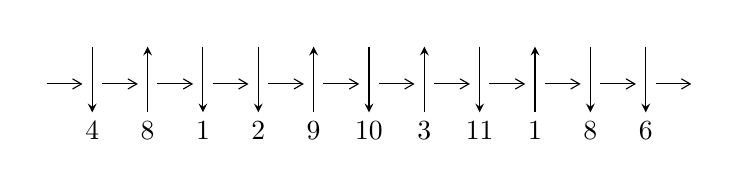
\begin{tikzpicture}[x=20pt, y=17pt]
	% nodes
	\node (C0) at (0, 0) {};
	\node (C1) at (1, 0) {};
	\node (C1U) at (1, +1) {};
	\node (C1D) at (1, -1) {4};

	\node (C2) at (2, 0) {};
	\node (C2U) at (2, +1) {};
	\node (C2D) at (2, -1) {8};

	\node (C3) at (3, 0) {};
	\node (C3U) at (3, +1) {};
	\node (C3D) at (3, -1) {1};

	\node (C4) at (4, 0) {};
	\node (C4U) at (4, +1) {};
	\node (C4D) at (4, -1) {2};

	\node (C5) at (5, 0) {};
	\node (C5U) at (5, +1) {};
	\node (C5D) at (5, -1) {9};

	\node (C6) at (6, 0) {};
	\node (C6U) at (6, +1) {};
	\node (C6D) at (6, -1) {10};

	\node (C7) at (7, 0) {};
	\node (C7U) at (7, +1) {};
	\node (C7D) at (7, -1) {3};

	\node (C8) at (8, 0) {};
	\node (C8U) at (8, +1) {};
	\node (C8D) at (8, -1) {11};

	\node (C9) at (9, 0) {};
	\node (C9U) at (9, +1) {};
	\node (C9D) at (9, -1) {1};

	\node (C10) at (10, 0) {};
	\node (C10U) at (10, +1) {};
	\node (C10D) at (10, -1) {8};

	\node (C11) at (11, 0) {};
	\node (C11U) at (11, +1) {};
	\node (C11D) at (11, -1) {6};
	\node (C12) at (12, 0) {};

	% arrows
	\draw[->,>={angle 60}]
	(C0) edge (C1) (C1) edge (C2) (C2) edge (C3) (C3) edge (C4) (C4) edge (C5) (C5) edge (C6) (C6) edge (C7) (C7) edge (C8) (C8) edge (C9) (C9) edge (C10) (C10) edge (C11) (C11) edge (C12) ;	\draw[->,>=stealth]
	(C1U) edge (C1D) (C2D) edge (C2U) (C3U) edge (C3D) (C4U) edge (C4D) (C5D) edge (C5U) (C6U) edge (C6D) (C7D) edge (C7U) (C8U) edge (C8D) (C9D) edge (C9U) (C10U) edge (C10D) (C11U) edge (C11D) ;
	\end{tikzpicture} \\
\hhline{~~} \\& 
\textbf{Solving Sequence} \\ \cline{2-2} 
 &
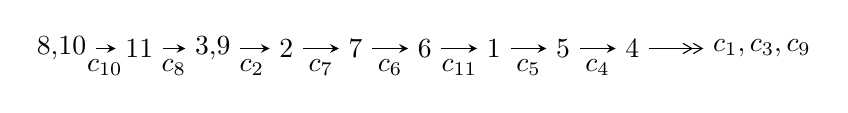
\begin{tikzpicture}[x=25pt, y=7pt]
	% node
	\node (A0) at (-1/8, 0) {8,10};
	\node (A1) at (1, 0) {11};
	\node (A2) at (33/16, 0) {3,9};
	\node (A3) at (25/8, 0) {2};
	\node (A4) at (33/8, 0) {7};
	\node (A5) at (41/8, 0) {6};
	\node (A6) at (49/8, 0) {1};
	\node (A7) at (57/8, 0) {5};
	\node (A8) at (65/8, 0) {4};
	\node (C1) at (1/2, -1) {$c_{10}$};
	\node (C2) at (3/2, -1) {$c_{8}$};
	\node (C3) at (21/8, -1) {$c_{2}$};
	\node (C4) at (29/8, -1) {$c_{7}$};
	\node (C5) at (37/8, -1) {$c_{6}$};
	\node (C6) at (45/8, -1) {$c_{11}$};
	\node (C7) at (53/8, -1) {$c_{5}$};
	\node (C8) at (61/8, -1) {$c_{4}$};
	\node (A9) at (10, 0) {$c_{1},c_{3},c_{9}$};

	% edge
	\draw[->,>=stealth]	
	(A0) edge (A1) (A1) edge (A2) (A2) edge (A3) (A3) edge (A4) (A4) edge (A5) (A5) edge (A6) (A6) edge (A7) (A7) edge (A8) ;
	\draw[->>,>={angle 60}]	
	(A8) edge (A9);
\end{tikzpicture} \\ 

\end{tabular} \\

\footnotetext{
The image of knot diagram is generated by the software ``\textbf{Draw programme}" developed by Andrew Bartholomew(\url{http://www.layer8.co.uk/maths/draw/index.htm\#Running-draw}), where we modified some parts for our purpose(\url{https://github.com/CATsTAILs/LinksPainter}).
}\phantom \\ \newline 
\centering \textbf{Ideals for irreducible components\footnotemark of $X_{\text{par}}$} 
 
\begin{align*}
I^u_{1}&=\langle 
- u^9+4 u^8-5 u^7-2 u^6+9 u^5-4 u^4-4 u^3+4 u^2+b- u,\\
\phantom{I^u_{1}}&\phantom{= \langle  }u^9-4 u^8+4 u^7+6 u^6-13 u^5+12 u^3-2 u^2+a-5 u,\\
\phantom{I^u_{1}}&\phantom{= \langle  }u^{11}-5 u^{10}+8 u^9+3 u^8-22 u^7+14 u^6+18 u^5-19 u^4-7 u^3+7 u^2+2 u+1\rangle \\
I^u_{2}&=\langle 
- u^4+u^3+u^2+b-1,\;a,\;u^5- u^4-2 u^3+u^2+u+1\rangle \\
I^u_{3}&=\langle 
a^4+2 a^2+b+2,\;a^5+a^4+2 a^3+a^2+a+1,\;u+1\rangle \\
I^u_{4}&=\langle 
- u^7+u^6- u^5-2 u^4+u^3+4 b+5 u+1,\\
\phantom{I^u_{4}}&\phantom{= \langle  }-9 u^9+17 u^8-44 u^7+5 u^6-38 u^5-78 u^4-4 u^3-207 u^2+16 a+7 u-113,\\
\phantom{I^u_{4}}&\phantom{= \langle  }u^{10}-2 u^9+5 u^8- u^7+3 u^6+8 u^5-2 u^4+19 u^3-6 u^2+8 u-1\rangle \\
\\
\end{align*}
\raggedright * 4 irreducible components of $\dim_{\mathbb{C}}=0$, with total 31 representations.\\
\footnotetext{All coefficients of polynomials are rational numbers. But the coefficients are sometimes approximated in decimal forms when there is not enough margin.}
\newpage
\renewcommand{\arraystretch}{1}
\centering \section*{I. $I^u_{1}= \langle - u^9+4 u^8+\cdots+b- u,\;u^9-4 u^8+\cdots+a-5 u,\;u^{11}-5 u^{10}+\cdots+2 u+1 \rangle$}
\flushleft \textbf{(i) Arc colorings}\\
\begin{tabular}{m{7pt} m{180pt} m{7pt} m{180pt} }
\flushright $a_{8}=$&$\begin{pmatrix}0\\u\end{pmatrix}$ \\
\flushright $a_{10}=$&$\begin{pmatrix}1\\0\end{pmatrix}$ \\
\flushright $a_{11}=$&$\begin{pmatrix}1\\u^2\end{pmatrix}$ \\
\flushright $a_{3}=$&$\begin{pmatrix}- u^9+4 u^8-4 u^7-6 u^6+13 u^5-12 u^3+2 u^2+5 u\\u^9-4 u^8+5 u^7+2 u^6-9 u^5+4 u^4+4 u^3-4 u^2+u\end{pmatrix}$ \\
\flushright $a_{9}=$&$\begin{pmatrix}- u\\- u^3+u\end{pmatrix}$ \\
\flushright $a_{2}=$&$\begin{pmatrix}- u^9+4 u^8-4 u^7-6 u^6+13 u^5-12 u^3+2 u^2+5 u\\- u^{10}+5 u^9-7 u^8-4 u^7+16 u^6-3 u^5-13 u^4+2 u^3+3 u^2+3 u+1\end{pmatrix}$ \\
\flushright $a_{7}=$&$\begin{pmatrix}u^2-1\\u^4-2 u^3+2 u\end{pmatrix}$ \\
\flushright $a_{6}=$&$\begin{pmatrix}u^4-2 u^3+u^2+2 u-1\\u^4-2 u^3+2 u\end{pmatrix}$ \\
\flushright $a_{1}=$&$\begin{pmatrix}- u^{10}+4 u^9-5 u^8-4 u^7+14 u^6-6 u^5-11 u^4+8 u^3+3 u^2-2 u+1\\- u^{10}+4 u^9-4 u^8-6 u^7+13 u^6-12 u^4+2 u^3+5 u^2\end{pmatrix}$ \\
\flushright $a_{5}=$&$\begin{pmatrix}u^8-2 u^7- u^6+6 u^5- u^4-6 u^3+2 u^2+2 u-1\\u^{10}-2 u^9-2 u^8+8 u^7- u^6-10 u^5+4 u^4+2 u^3- u^2+2 u\end{pmatrix}$ \\
\flushright $a_{4}=$&$\begin{pmatrix}u^{10}-4 u^9+5 u^8+4 u^7-14 u^6+6 u^5+11 u^4-8 u^3-3 u^2+2 u-1\\u^{10}-3 u^9- u^8+14 u^7-12 u^6-15 u^5+21 u^4+6 u^3-11 u^2- u-1\end{pmatrix}$\\ \flushright $a_{4}=$&$\begin{pmatrix}u^{10}-4 u^9+5 u^8+4 u^7-14 u^6+6 u^5+11 u^4-8 u^3-3 u^2+2 u-1\\u^{10}-3 u^9- u^8+14 u^7-12 u^6-15 u^5+21 u^4+6 u^3-11 u^2- u-1\end{pmatrix}$\\&\end{tabular}
\flushleft \textbf{(ii) Obstruction class $= -1$}\\~\\
\flushleft \textbf{(iii) Cusp Shapes $= 4 u^{10}-16 u^9+20 u^8+8 u^7-24 u^6-16 u^5+28 u^4+32 u^3-28 u^2-24 u-6$}\\~\\
\newpage\renewcommand{\arraystretch}{1}
\flushleft \textbf{(iv) u-Polynomials at the component}\newline \\
\begin{tabular}{m{50pt}|m{274pt}}
Crossings & \hspace{64pt}u-Polynomials at each crossing \\
\hline $$\begin{aligned}c_{1},c_{3},c_{4}\\c_{8},c_{10}\end{aligned}$$&$\begin{aligned}
&u^{11}-5 u^{10}+\cdots+2 u+1
\end{aligned}$\\
\hline $$\begin{aligned}c_{2},c_{7},c_{9}\end{aligned}$$&$\begin{aligned}
&u^{11}+u^{10}+\cdots+2 u+1
\end{aligned}$\\
\hline $$\begin{aligned}c_{5}\end{aligned}$$&$\begin{aligned}
&u^{11}- u^{10}+3 u^8+12 u^7+10 u^6-6 u^5-33 u^4-31 u^3-33 u^2-10 u-11
\end{aligned}$\\
\hline $$\begin{aligned}c_{6}\end{aligned}$$&$\begin{aligned}
&u^{11}+u^{10}+\cdots-33 u^2-27
\end{aligned}$\\
\hline $$\begin{aligned}c_{11}\end{aligned}$$&$\begin{aligned}
&u^{11}- u^{10}+u^8+8 u^7-12 u^6+8 u^5+3 u^4+3 u^3-3 u^2+1
\end{aligned}$\\
\hline
\end{tabular}\\~\\
\newpage\renewcommand{\arraystretch}{1}
\flushleft \textbf{(v) Riley Polynomials at the component}\newline \\
\begin{tabular}{m{50pt}|m{274pt}}
Crossings & \hspace{64pt}Riley Polynomials at each crossing \\
\hline $$\begin{aligned}c_{1},c_{3},c_{4}\\c_{8},c_{10}\end{aligned}$$&$\begin{aligned}
&y^{11}-9 y^{10}+\cdots-10 y-1
\end{aligned}$\\
\hline $$\begin{aligned}c_{2},c_{7},c_{9}\end{aligned}$$&$\begin{aligned}
&y^{11}-9 y^{10}+\cdots-2 y-1
\end{aligned}$\\
\hline $$\begin{aligned}c_{5}\end{aligned}$$&$\begin{aligned}
&y^{11}- y^{10}+\cdots-626 y-121
\end{aligned}$\\
\hline $$\begin{aligned}c_{6}\end{aligned}$$&$\begin{aligned}
&y^{11}+15 y^{10}+\cdots-1782 y-729
\end{aligned}$\\
\hline $$\begin{aligned}c_{11}\end{aligned}$$&$\begin{aligned}
&y^{11}- y^{10}+\cdots+6 y-1
\end{aligned}$\\
\hline
\end{tabular}\\~\\
\newpage\flushleft \textbf{(vi) Complex Volumes and Cusp Shapes}
$$\begin{array}{c|c|c}  
\text{Solutions to }I^u_{1}& \I (\text{vol} + \sqrt{-1}CS) & \text{Cusp shape}\\
 \hline 
\begin{aligned}
u &= -1.07566\phantom{ +0.000000I} \\
a &= -0.382088\phantom{ +0.000000I} \\
b &= -6.69648\phantom{ +0.000000I}\end{aligned}
 & -3.78211\phantom{ +0.000000I} & \phantom{-}32.5960\phantom{ +0.000000I} \\ \hline\begin{aligned}
u &= -0.832306 + 0.202239 I \\
a &= -0.362795 + 0.658644 I \\
b &= -1.76349 - 0.21001 I\end{aligned}
 & -2.76312 + 1.08944 I & -13.75530 + 1.30535 I \\ \hline\begin{aligned}
u &= -0.832306 - 0.202239 I \\
a &= -0.362795 - 0.658644 I \\
b &= -1.76349 + 0.21001 I\end{aligned}
 & -2.76312 - 1.08944 I & -13.75530 - 1.30535 I \\ \hline\begin{aligned}
u &= \phantom{-}1.263210 + 0.139301 I \\
a &= \phantom{-}0.158505 - 0.711489 I \\
b &= \phantom{-}0.009586 + 0.293616 I\end{aligned}
 & -8.16883 - 4.71969 I & -15.8344 + 7.6612 I \\ \hline\begin{aligned}
u &= \phantom{-}1.263210 - 0.139301 I \\
a &= \phantom{-}0.158505 + 0.711489 I \\
b &= \phantom{-}0.009586 - 0.293616 I\end{aligned}
 & -8.16883 + 4.71969 I & -15.8344 - 7.6612 I \\ \hline\begin{aligned}
u &= \phantom{-}1.31469 + 0.95832 I \\
a &= -0.606321 + 1.088860 I \\
b &= -0.10260 - 1.75202 I\end{aligned}
 & \phantom{-}7.84139 - 5.06071 I & -4.48302 + 2.40182 I \\ \hline\begin{aligned}
u &= \phantom{-}1.31469 - 0.95832 I \\
a &= -0.606321 - 1.088860 I \\
b &= -0.10260 + 1.75202 I\end{aligned}
 & \phantom{-}7.84139 + 5.06071 I & -4.48302 - 2.40182 I \\ \hline\begin{aligned}
u &= -0.113634 + 0.293281 I \\
a &= -1.09164 + 1.49222 I \\
b &= \phantom{-}0.322788 + 0.550650 I\end{aligned}
 & \phantom{-}0.003691 + 1.266700 I & -0.27668 - 5.30833 I \\ \hline\begin{aligned}
u &= -0.113634 - 0.293281 I \\
a &= -1.09164 - 1.49222 I \\
b &= \phantom{-}0.322788 - 0.550650 I\end{aligned}
 & \phantom{-}0.003691 - 1.266700 I & -0.27668 + 5.30833 I \\ \hline\begin{aligned}
u &= \phantom{-}1.40586 + 1.00997 I \\
a &= \phantom{-}0.593293 - 1.135200 I \\
b &= \phantom{-}0.38195 + 1.94651 I\end{aligned}
 & \phantom{-}7.4453 - 12.4339 I & -4.94880 + 5.95992 I\\
 \hline 
 \end{array}$$\newpage$$\begin{array}{c|c|c}  
\text{Solutions to }I^u_{1}& \I (\text{vol} + \sqrt{-1}CS) & \text{Cusp shape}\\
 \hline 
\begin{aligned}
u &= \phantom{-}1.40586 - 1.00997 I \\
a &= \phantom{-}0.593293 + 1.135200 I \\
b &= \phantom{-}0.38195 - 1.94651 I\end{aligned}
 & \phantom{-}7.4453 + 12.4339 I & -4.94880 - 5.95992 I\\
 \hline 
 \end{array}$$\newpage\newpage\renewcommand{\arraystretch}{1}
\centering \section*{II. $I^u_{2}= \langle - u^4+u^3+u^2+b-1,\;a,\;u^5- u^4-2 u^3+u^2+u+1 \rangle$}
\flushleft \textbf{(i) Arc colorings}\\
\begin{tabular}{m{7pt} m{180pt} m{7pt} m{180pt} }
\flushright $a_{8}=$&$\begin{pmatrix}0\\u\end{pmatrix}$ \\
\flushright $a_{10}=$&$\begin{pmatrix}1\\0\end{pmatrix}$ \\
\flushright $a_{11}=$&$\begin{pmatrix}1\\u^2\end{pmatrix}$ \\
\flushright $a_{3}=$&$\begin{pmatrix}0\\u^4- u^3- u^2+1\end{pmatrix}$ \\
\flushright $a_{9}=$&$\begin{pmatrix}- u\\- u^3+u\end{pmatrix}$ \\
\flushright $a_{2}=$&$\begin{pmatrix}0\\u^4- u^3- u^2+1\end{pmatrix}$ \\
\flushright $a_{7}=$&$\begin{pmatrix}0\\u\end{pmatrix}$ \\
\flushright $a_{6}=$&$\begin{pmatrix}u\\u\end{pmatrix}$ \\
\flushright $a_{1}=$&$\begin{pmatrix}- u^4+u^2+1\\- u^4+2 u^2\end{pmatrix}$ \\
\flushright $a_{5}=$&$\begin{pmatrix}u^4- u^2-1\\u^4-2 u^2\end{pmatrix}$ \\
\flushright $a_{4}=$&$\begin{pmatrix}u^4- u^2-1\\2 u^4- u^3-3 u^2+1\end{pmatrix}$\\ \flushright $a_{4}=$&$\begin{pmatrix}u^4- u^2-1\\2 u^4- u^3-3 u^2+1\end{pmatrix}$\\&\end{tabular}
\flushleft \textbf{(ii) Obstruction class $= 1$}\\~\\
\flushleft \textbf{(iii) Cusp Shapes $= -3 u^4+7 u^3+2 u^2-6 u-7$}\\~\\
\newpage\renewcommand{\arraystretch}{1}
\flushleft \textbf{(iv) u-Polynomials at the component}\newline \\
\begin{tabular}{m{50pt}|m{274pt}}
Crossings & \hspace{64pt}u-Polynomials at each crossing \\
\hline $$\begin{aligned}c_{1}\end{aligned}$$&$\begin{aligned}
&(u-1)^5
\end{aligned}$\\
\hline $$\begin{aligned}c_{2},c_{7}\end{aligned}$$&$\begin{aligned}
&u^5
\end{aligned}$\\
\hline $$\begin{aligned}c_{3},c_{4}\end{aligned}$$&$\begin{aligned}
&(u+1)^5
\end{aligned}$\\
\hline $$\begin{aligned}c_{5},c_{9}\end{aligned}$$&$\begin{aligned}
&u^5- u^4+2 u^3- u^2+u-1
\end{aligned}$\\
\hline $$\begin{aligned}c_{6},c_{8}\end{aligned}$$&$\begin{aligned}
&u^5+u^4-2 u^3- u^2+u-1
\end{aligned}$\\
\hline $$\begin{aligned}c_{10}\end{aligned}$$&$\begin{aligned}
&u^5- u^4-2 u^3+u^2+u+1
\end{aligned}$\\
\hline $$\begin{aligned}c_{11}\end{aligned}$$&$\begin{aligned}
&u^5+3 u^4+4 u^3+u^2- u-1
\end{aligned}$\\
\hline
\end{tabular}\\~\\
\newpage\renewcommand{\arraystretch}{1}
\flushleft \textbf{(v) Riley Polynomials at the component}\newline \\
\begin{tabular}{m{50pt}|m{274pt}}
Crossings & \hspace{64pt}Riley Polynomials at each crossing \\
\hline $$\begin{aligned}c_{1},c_{3},c_{4}\end{aligned}$$&$\begin{aligned}
&(y-1)^5
\end{aligned}$\\
\hline $$\begin{aligned}c_{2},c_{7}\end{aligned}$$&$\begin{aligned}
&y^5
\end{aligned}$\\
\hline $$\begin{aligned}c_{5},c_{9}\end{aligned}$$&$\begin{aligned}
&y^5+3 y^4+4 y^3+y^2- y-1
\end{aligned}$\\
\hline $$\begin{aligned}c_{6},c_{8},c_{10}\end{aligned}$$&$\begin{aligned}
&y^5-5 y^4+8 y^3-3 y^2- y-1
\end{aligned}$\\
\hline $$\begin{aligned}c_{11}\end{aligned}$$&$\begin{aligned}
&y^5- y^4+8 y^3-3 y^2+3 y-1
\end{aligned}$\\
\hline
\end{tabular}\\~\\
\newpage\flushleft \textbf{(vi) Complex Volumes and Cusp Shapes}
$$\begin{array}{c|c|c}  
\text{Solutions to }I^u_{2}& \I (\text{vol} + \sqrt{-1}CS) & \text{Cusp shape}\\
 \hline 
\begin{aligned}
u &= -1.21774\phantom{ +0.000000I} \\
a &= \phantom{-0.000000 } 0 \\
b &= \phantom{-}3.52181\phantom{ +0.000000I}\end{aligned}
 & -4.04602\phantom{ +0.000000I} & -15.9650\phantom{ +0.000000I} \\ \hline\begin{aligned}
u &= -0.309916 + 0.549911 I \\
a &= \phantom{-0.000000 } 0 \\
b &= \phantom{-}0.881366 + 0.489365 I\end{aligned}
 & -1.97403 + 1.53058 I & -3.57269 - 4.45807 I \\ \hline\begin{aligned}
u &= -0.309916 - 0.549911 I \\
a &= \phantom{-0.000000 } 0 \\
b &= \phantom{-}0.881366 - 0.489365 I\end{aligned}
 & -1.97403 - 1.53058 I & -3.57269 + 4.45807 I \\ \hline\begin{aligned}
u &= \phantom{-}1.41878 + 0.21917 I \\
a &= \phantom{-0.000000 } 0 \\
b &= -0.142272 + 0.509071 I\end{aligned}
 & -7.51750 - 4.40083 I & -3.44484 + 1.78781 I \\ \hline\begin{aligned}
u &= \phantom{-}1.41878 - 0.21917 I \\
a &= \phantom{-0.000000 } 0 \\
b &= -0.142272 - 0.509071 I\end{aligned}
 & -7.51750 + 4.40083 I & -3.44484 - 1.78781 I\\
 \hline 
 \end{array}$$\newpage\newpage\renewcommand{\arraystretch}{1}
\centering \section*{III. $I^u_{3}= \langle a^4+2 a^2+b+2,\;a^5+a^4+2 a^3+a^2+a+1,\;u+1 \rangle$}
\flushleft \textbf{(i) Arc colorings}\\
\begin{tabular}{m{7pt} m{180pt} m{7pt} m{180pt} }
\flushright $a_{8}=$&$\begin{pmatrix}0\\-1\end{pmatrix}$ \\
\flushright $a_{10}=$&$\begin{pmatrix}1\\0\end{pmatrix}$ \\
\flushright $a_{11}=$&$\begin{pmatrix}1\\1\end{pmatrix}$ \\
\flushright $a_{3}=$&$\begin{pmatrix}a\\- a^4-2 a^2-2\end{pmatrix}$ \\
\flushright $a_{9}=$&$\begin{pmatrix}1\\0\end{pmatrix}$ \\
\flushright $a_{2}=$&$\begin{pmatrix}a\\- a^4-2 a^2+a-2\end{pmatrix}$ \\
\flushright $a_{7}=$&$\begin{pmatrix}a^2\\a^4+a^2- a\end{pmatrix}$ \\
\flushright $a_{6}=$&$\begin{pmatrix}a^4+2 a^2- a\\a^4+a^2- a\end{pmatrix}$ \\
\flushright $a_{1}=$&$\begin{pmatrix}- a^4\\0\end{pmatrix}$ \\
\flushright $a_{5}=$&$\begin{pmatrix}a^2\\a^4+a^2- a\end{pmatrix}$ \\
\flushright $a_{4}=$&$\begin{pmatrix}- a^4\\- a^4-2 a^2-2\end{pmatrix}$\\ \flushright $a_{4}=$&$\begin{pmatrix}- a^4\\- a^4-2 a^2-2\end{pmatrix}$\\&\end{tabular}
\flushleft \textbf{(ii) Obstruction class $= 1$}\\~\\
\flushleft \textbf{(iii) Cusp Shapes $= -4 a^4-3 a^3-11 a^2-2 a-11$}\\~\\
\newpage\renewcommand{\arraystretch}{1}
\flushleft \textbf{(iv) u-Polynomials at the component}\newline \\
\begin{tabular}{m{50pt}|m{274pt}}
Crossings & \hspace{64pt}u-Polynomials at each crossing \\
\hline $$\begin{aligned}c_{1}\end{aligned}$$&$\begin{aligned}
&u^5+u^4-2 u^3- u^2+u-1
\end{aligned}$\\
\hline $$\begin{aligned}c_{2}\end{aligned}$$&$\begin{aligned}
&u^5- u^4+2 u^3- u^2+u-1
\end{aligned}$\\
\hline $$\begin{aligned}c_{3},c_{4}\end{aligned}$$&$\begin{aligned}
&u^5- u^4-2 u^3+u^2+u+1
\end{aligned}$\\
\hline $$\begin{aligned}c_{5},c_{6}\end{aligned}$$&$\begin{aligned}
&u^5- u^4- u^3+4 u^2-3 u+1
\end{aligned}$\\
\hline $$\begin{aligned}c_{7}\end{aligned}$$&$\begin{aligned}
&u^5+u^4+2 u^3+u^2+u+1
\end{aligned}$\\
\hline $$\begin{aligned}c_{8}\end{aligned}$$&$\begin{aligned}
&(u-1)^5
\end{aligned}$\\
\hline $$\begin{aligned}c_{9}\end{aligned}$$&$\begin{aligned}
&u^5
\end{aligned}$\\
\hline $$\begin{aligned}c_{10}\end{aligned}$$&$\begin{aligned}
&(u+1)^5
\end{aligned}$\\
\hline $$\begin{aligned}c_{11}\end{aligned}$$&$\begin{aligned}
&u^5-3 u^4+4 u^3- u^2- u+1
\end{aligned}$\\
\hline
\end{tabular}\\~\\
\newpage\renewcommand{\arraystretch}{1}
\flushleft \textbf{(v) Riley Polynomials at the component}\newline \\
\begin{tabular}{m{50pt}|m{274pt}}
Crossings & \hspace{64pt}Riley Polynomials at each crossing \\
\hline $$\begin{aligned}c_{1},c_{3},c_{4}\end{aligned}$$&$\begin{aligned}
&y^5-5 y^4+8 y^3-3 y^2- y-1
\end{aligned}$\\
\hline $$\begin{aligned}c_{2},c_{7}\end{aligned}$$&$\begin{aligned}
&y^5+3 y^4+4 y^3+y^2- y-1
\end{aligned}$\\
\hline $$\begin{aligned}c_{5},c_{6}\end{aligned}$$&$\begin{aligned}
&y^5-3 y^4+3 y^3-8 y^2+y-1
\end{aligned}$\\
\hline $$\begin{aligned}c_{8},c_{10}\end{aligned}$$&$\begin{aligned}
&(y-1)^5
\end{aligned}$\\
\hline $$\begin{aligned}c_{9}\end{aligned}$$&$\begin{aligned}
&y^5
\end{aligned}$\\
\hline $$\begin{aligned}c_{11}\end{aligned}$$&$\begin{aligned}
&y^5- y^4+8 y^3-3 y^2+3 y-1
\end{aligned}$\\
\hline
\end{tabular}\\~\\
\newpage\flushleft \textbf{(vi) Complex Volumes and Cusp Shapes}
$$\begin{array}{c|c|c}  
\text{Solutions to }I^u_{3}& \I (\text{vol} + \sqrt{-1}CS) & \text{Cusp shape}\\
 \hline 
\begin{aligned}
u &= -1.00000\phantom{ +0.000000I} \\
a &= \phantom{-}0.339110 + 0.822375 I \\
b &= -0.881366 - 0.489365 I\end{aligned}
 & -1.97403 + 1.53058 I & -3.57269 - 4.45807 I \\ \hline\begin{aligned}
u &= -1.00000\phantom{ +0.000000I} \\
a &= \phantom{-}0.339110 - 0.822375 I \\
b &= -0.881366 + 0.489365 I\end{aligned}
 & -1.97403 - 1.53058 I & -3.57269 + 4.45807 I \\ \hline\begin{aligned}
u &= -1.00000\phantom{ +0.000000I} \\
a &= -0.766826\phantom{ +0.000000I} \\
b &= -3.52181\phantom{ +0.000000I}\end{aligned}
 & -4.04602\phantom{ +0.000000I} & -15.9650\phantom{ +0.000000I} \\ \hline\begin{aligned}
u &= -1.00000\phantom{ +0.000000I} \\
a &= -0.455697 + 1.200150 I \\
b &= \phantom{-}0.142272 - 0.509071 I\end{aligned}
 & -7.51750 - 4.40083 I & -3.44484 + 1.78781 I \\ \hline\begin{aligned}
u &= -1.00000\phantom{ +0.000000I} \\
a &= -0.455697 - 1.200150 I \\
b &= \phantom{-}0.142272 + 0.509071 I\end{aligned}
 & -7.51750 + 4.40083 I & -3.44484 - 1.78781 I\\
 \hline 
 \end{array}$$\newpage\newpage\renewcommand{\arraystretch}{1}
\centering \section*{IV. $I^u_{4}= \langle - u^7+u^6- u^5-2 u^4+u^3+4 b+5 u+1,\;-9 u^9+17 u^8+\cdots+16 a-113,\;u^{10}-2 u^9+\cdots+8 u-1 \rangle$}
\flushleft \textbf{(i) Arc colorings}\\
\begin{tabular}{m{7pt} m{180pt} m{7pt} m{180pt} }
\flushright $a_{8}=$&$\begin{pmatrix}0\\u\end{pmatrix}$ \\
\flushright $a_{10}=$&$\begin{pmatrix}1\\0\end{pmatrix}$ \\
\flushright $a_{11}=$&$\begin{pmatrix}1\\u^2\end{pmatrix}$ \\
\flushright $a_{3}=$&$\begin{pmatrix}0.562500 u^{9}-1.06250 u^{8}+\cdots-0.437500 u+7.06250\\\frac{1}{4} u^7-\frac{1}{4} u^6+\cdots-\frac{5}{4} u-\frac{1}{4}\end{pmatrix}$ \\
\flushright $a_{9}=$&$\begin{pmatrix}- u\\- u^3+u\end{pmatrix}$ \\
\flushright $a_{2}=$&$\begin{pmatrix}0.562500 u^{9}-1.06250 u^{8}+\cdots-0.437500 u+7.06250\\0.0625000 u^{9}-0.0625000 u^{8}+\cdots-1.18750 u-0.187500\end{pmatrix}$ \\
\flushright $a_{7}=$&$\begin{pmatrix}-\frac{3}{2} u^9+\frac{19}{8} u^8+\cdots+u-\frac{53}{8}\\0.312500 u^{9}-0.437500 u^{8}+\cdots+0.0625000 u+0.437500\end{pmatrix}$ \\
\flushright $a_{6}=$&$\begin{pmatrix}-1.18750 u^{9}+1.93750 u^{8}+\cdots+1.06250 u-6.18750\\0.312500 u^{9}-0.437500 u^{8}+\cdots+0.0625000 u+0.437500\end{pmatrix}$ \\
\flushright $a_{1}=$&$\begin{pmatrix}-\frac{1}{4} u^9+\frac{1}{2} u^8+\cdots+\frac{3}{2} u-\frac{13}{4}\\\frac{1}{4} u^8-\frac{1}{2} u^7+\cdots+u+\frac{1}{4}\end{pmatrix}$ \\
\flushright $a_{5}=$&$\begin{pmatrix}- u^9+\frac{11}{8} u^8+\cdots-\frac{5}{2} u-\frac{45}{8}\\-0.437500 u^{9}+0.312500 u^{8}+\cdots+5.31250 u-0.312500\end{pmatrix}$ \\
\flushright $a_{4}=$&$\begin{pmatrix}\frac{1}{4} u^9-\frac{1}{2} u^8+\cdots-\frac{3}{2} u+\frac{13}{4}\\-\frac{1}{4} u^8+\frac{1}{4} u^7+\cdots+\frac{5}{4} u^2+\frac{1}{4} u\end{pmatrix}$\\ \flushright $a_{4}=$&$\begin{pmatrix}\frac{1}{4} u^9-\frac{1}{2} u^8+\cdots-\frac{3}{2} u+\frac{13}{4}\\-\frac{1}{4} u^8+\frac{1}{4} u^7+\cdots+\frac{5}{4} u^2+\frac{1}{4} u\end{pmatrix}$\\&\end{tabular}
\flushleft \textbf{(ii) Obstruction class $= -1$}\\~\\
\flushleft \textbf{(iii) Cusp Shapes $= -\frac{1}{4} u^9+\frac{7}{8} u^8-\frac{9}{4} u^7+2 u^6-\frac{3}{8} u^5-\frac{23}{8} u^4+\frac{33}{8} u^3-\frac{35}{8} u^2+\frac{31}{4} u-\frac{37}{8}$}\\~\\
\newpage\renewcommand{\arraystretch}{1}
\flushleft \textbf{(iv) u-Polynomials at the component}\newline \\
\begin{tabular}{m{50pt}|m{274pt}}
Crossings & \hspace{64pt}u-Polynomials at each crossing \\
\hline $$\begin{aligned}c_{1},c_{3},c_{4}\\c_{8},c_{10}\end{aligned}$$&$\begin{aligned}
&u^{10}-2 u^9+5 u^8- u^7+3 u^6+8 u^5-2 u^4+19 u^3-6 u^2+8 u-1
\end{aligned}$\\
\hline $$\begin{aligned}c_{2},c_{7},c_{9}\end{aligned}$$&$\begin{aligned}
&u^{10}+u^9+\cdots+160 u+32
\end{aligned}$\\
\hline $$\begin{aligned}c_{5}\end{aligned}$$&$\begin{aligned}
&u^{10}-10 u^8+43 u^6+17 u^5-35 u^4+46 u^3+64 u^2-38 u-29
\end{aligned}$\\
\hline $$\begin{aligned}c_{6}\end{aligned}$$&$\begin{aligned}
&u^{10}+2 u^9+\cdots-100 u-43
\end{aligned}$\\
\hline $$\begin{aligned}c_{11}\end{aligned}$$&$\begin{aligned}
&(u^5- u^4+u^2+u-1)^2
\end{aligned}$\\
\hline
\end{tabular}\\~\\
\newpage\renewcommand{\arraystretch}{1}
\flushleft \textbf{(v) Riley Polynomials at the component}\newline \\
\begin{tabular}{m{50pt}|m{274pt}}
Crossings & \hspace{64pt}Riley Polynomials at each crossing \\
\hline $$\begin{aligned}c_{1},c_{3},c_{4}\\c_{8},c_{10}\end{aligned}$$&$\begin{aligned}
&y^{10}+6 y^9+\cdots-52 y+1
\end{aligned}$\\
\hline $$\begin{aligned}c_{2},c_{7},c_{9}\end{aligned}$$&$\begin{aligned}
&y^{10}-21 y^9+\cdots-9728 y+1024
\end{aligned}$\\
\hline $$\begin{aligned}c_{5}\end{aligned}$$&$\begin{aligned}
&y^{10}-20 y^9+\cdots-5156 y+841
\end{aligned}$\\
\hline $$\begin{aligned}c_{6}\end{aligned}$$&$\begin{aligned}
&y^{10}+20 y^9+\cdots-13440 y+1849
\end{aligned}$\\
\hline $$\begin{aligned}c_{11}\end{aligned}$$&$\begin{aligned}
&(y^5- y^4+4 y^3-3 y^2+3 y-1)^2
\end{aligned}$\\
\hline
\end{tabular}\\~\\
\newpage\flushleft \textbf{(vi) Complex Volumes and Cusp Shapes}
$$\begin{array}{c|c|c}  
\text{Solutions to }I^u_{4}& \I (\text{vol} + \sqrt{-1}CS) & \text{Cusp shape}\\
 \hline 
\begin{aligned}
u &= -0.394402 + 1.113210 I \\
a &= -0.721708 - 0.484512 I \\
b &= -0.233677 + 0.885557 I\end{aligned}
 & \phantom{-}0.17487 + 2.21397 I & -2.88087 - 4.04855 I \\ \hline\begin{aligned}
u &= -0.394402 - 1.113210 I \\
a &= -0.721708 + 0.484512 I \\
b &= -0.233677 - 0.885557 I\end{aligned}
 & \phantom{-}0.17487 - 2.21397 I & -2.88087 + 4.04855 I \\ \hline\begin{aligned}
u &= \phantom{-}0.124008 + 0.699342 I \\
a &= \phantom{-}1.91026 + 1.28243 I \\
b &= -0.233677 - 0.885557 I\end{aligned}
 & \phantom{-}0.17487 - 2.21397 I & -2.88087 + 4.04855 I \\ \hline\begin{aligned}
u &= \phantom{-}0.124008 - 0.699342 I \\
a &= \phantom{-}1.91026 - 1.28243 I \\
b &= -0.233677 + 0.885557 I\end{aligned}
 & \phantom{-}0.17487 + 2.21397 I & -2.88087 - 4.04855 I \\ \hline\begin{aligned}
u &= -1.30598\phantom{ +0.000000I} \\
a &= -0.276456\phantom{ +0.000000I} \\
b &= -0.416284\phantom{ +0.000000I}\end{aligned}
 & -2.52712\phantom{ +0.000000I} & -3.66490\phantom{ +0.000000I} \\ \hline\begin{aligned}
u &= \phantom{-}0.93349 + 1.31744 I \\
a &= -0.80555 + 1.36977 I \\
b &= -0.05818 - 1.69128 I\end{aligned}
 & \phantom{-}9.31336 - 3.33174 I & -3.28666 + 2.53508 I \\ \hline\begin{aligned}
u &= \phantom{-}0.93349 - 1.31744 I \\
a &= -0.80555 - 1.36977 I \\
b &= -0.05818 + 1.69128 I\end{aligned}
 & \phantom{-}9.31336 + 3.33174 I & -3.28666 - 2.53508 I \\ \hline\begin{aligned}
u &= \phantom{-}0.92355 + 1.51424 I \\
a &= \phantom{-}0.638018 - 1.084890 I \\
b &= -0.05818 + 1.69128 I\end{aligned}
 & \phantom{-}9.31336 + 3.33174 I & -3.28666 - 2.53508 I \\ \hline\begin{aligned}
u &= \phantom{-}0.92355 - 1.51424 I \\
a &= \phantom{-}0.638018 + 1.084890 I \\
b &= -0.05818 - 1.69128 I\end{aligned}
 & \phantom{-}9.31336 - 3.33174 I & -3.28666 + 2.53508 I \\ \hline\begin{aligned}
u &= \phantom{-}0.132691\phantom{ +0.000000I} \\
a &= \phantom{-}7.23443\phantom{ +0.000000I} \\
b &= -0.416284\phantom{ +0.000000I}\end{aligned}
 & -2.52712\phantom{ +0.000000I} & -3.66490\phantom{ +0.000000I}\\
 \hline 
 \end{array}$$\newpage
\newpage\renewcommand{\arraystretch}{1}
\centering \section*{ V. u-Polynomials}
\begin{tabular}{m{50pt}|m{274pt}}
Crossings & \hspace{64pt}u-Polynomials at each crossing \\
\hline $$\begin{aligned}c_{1},c_{8}\end{aligned}$$&$\begin{aligned}
&(u-1)^5(u^5+u^4-2 u^3- u^2+u-1)\\
&\cdot(u^{10}-2 u^9+5 u^8- u^7+3 u^6+8 u^5-2 u^4+19 u^3-6 u^2+8 u-1)\\
&\cdot(u^{11}-5 u^{10}+\cdots+2 u+1)
\end{aligned}$\\
\hline $$\begin{aligned}c_{2},c_{9}\end{aligned}$$&$\begin{aligned}
&u^5(u^5- u^4+\cdots+u-1)(u^{10}+u^9+\cdots+160 u+32)\\
&\cdot(u^{11}+u^{10}+\cdots+2 u+1)
\end{aligned}$\\
\hline $$\begin{aligned}c_{3},c_{4},c_{10}\end{aligned}$$&$\begin{aligned}
&(u+1)^5(u^5- u^4-2 u^3+u^2+u+1)\\
&\cdot(u^{10}-2 u^9+5 u^8- u^7+3 u^6+8 u^5-2 u^4+19 u^3-6 u^2+8 u-1)\\
&\cdot(u^{11}-5 u^{10}+\cdots+2 u+1)
\end{aligned}$\\
\hline $$\begin{aligned}c_{5}\end{aligned}$$&$\begin{aligned}
&(u^5- u^4- u^3+4 u^2-3 u+1)(u^5- u^4+2 u^3- u^2+u-1)\\
&\cdot(u^{10}-10 u^8+43 u^6+17 u^5-35 u^4+46 u^3+64 u^2-38 u-29)\\
&\cdot(u^{11}- u^{10}+3 u^8+12 u^7+10 u^6-6 u^5-33 u^4-31 u^3-33 u^2-10 u-11)
\end{aligned}$\\
\hline $$\begin{aligned}c_{6}\end{aligned}$$&$\begin{aligned}
&(u^5- u^4- u^3+4 u^2-3 u+1)(u^5+u^4-2 u^3- u^2+u-1)\\
&\cdot(u^{10}+2 u^9+\cdots-100 u-43)(u^{11}+u^{10}+\cdots-33 u^2-27)
\end{aligned}$\\
\hline $$\begin{aligned}c_{7}\end{aligned}$$&$\begin{aligned}
&u^5(u^5+u^4+\cdots+u+1)(u^{10}+u^9+\cdots+160 u+32)\\
&\cdot(u^{11}+u^{10}+\cdots+2 u+1)
\end{aligned}$\\
\hline $$\begin{aligned}c_{11}\end{aligned}$$&$\begin{aligned}
&(u^5-3 u^4+4 u^3- u^2- u+1)(u^5- u^4+u^2+u-1)^2\\
&\cdot(u^5+3 u^4+4 u^3+u^2- u-1)\\
&\cdot(u^{11}- u^{10}+u^8+8 u^7-12 u^6+8 u^5+3 u^4+3 u^3-3 u^2+1)
\end{aligned}$\\
\hline
\end{tabular}\newpage\renewcommand{\arraystretch}{1}
\centering \section*{ VI. Riley Polynomials}
\begin{tabular}{m{50pt}|m{274pt}}
Crossings & \hspace{64pt}Riley Polynomials at each crossing \\
\hline $$\begin{aligned}c_{1},c_{3},c_{4}\\c_{8},c_{10}\end{aligned}$$&$\begin{aligned}
&((y-1)^5)(y^5-5 y^4+\cdots- y-1)(y^{10}+6 y^9+\cdots-52 y+1)\\
&\cdot(y^{11}-9 y^{10}+\cdots-10 y-1)
\end{aligned}$\\
\hline $$\begin{aligned}c_{2},c_{7},c_{9}\end{aligned}$$&$\begin{aligned}
&y^5(y^5+3 y^4+\cdots- y-1)(y^{10}-21 y^{9}+\cdots-9728 y+1024)\\
&\cdot(y^{11}-9 y^{10}+\cdots-2 y-1)
\end{aligned}$\\
\hline $$\begin{aligned}c_{5}\end{aligned}$$&$\begin{aligned}
&(y^5-3 y^4+3 y^3-8 y^2+y-1)(y^5+3 y^4+4 y^3+y^2- y-1)\\
&\cdot(y^{10}-20 y^9+\cdots-5156 y+841)(y^{11}- y^{10}+\cdots-626 y-121)
\end{aligned}$\\
\hline $$\begin{aligned}c_{6}\end{aligned}$$&$\begin{aligned}
&(y^5-5 y^4+8 y^3-3 y^2- y-1)(y^5-3 y^4+3 y^3-8 y^2+y-1)\\
&\cdot(y^{10}+20 y^9+\cdots-13440 y+1849)\\
&\cdot(y^{11}+15 y^{10}+\cdots-1782 y-729)
\end{aligned}$\\
\hline $$\begin{aligned}c_{11}\end{aligned}$$&$\begin{aligned}
&(y^5- y^4+4 y^3-3 y^2+3 y-1)^2(y^5- y^4+8 y^3-3 y^2+3 y-1)^2\\
&\cdot(y^{11}- y^{10}+\cdots+6 y-1)
\end{aligned}$\\
\hline
\end{tabular}
\vskip 2pc
\end{document}